\chapter{P$\mathrm{_N}$ Method and Diffusion}
\label{lec:pn_method_and_diffusion}

We continue in this lecture our treatment of the integro-differential form of the transport equation.  Here, we turn to expansion of the angular variable in an orthogonal basis, the well-known Legendre polynomials in slab geometry and the spherical harmonics in multidimensional settings.  This approach is typically referred to generically as the $P_N$ method, which is the common symbol for the Legendre polynomials.  We'll first start with a brief discussion of anisotropic scattering and how it can be handled using orthogonal expansions.  We'll then derive the $P_N$ equations for slab geometry, show how one formally arrives at the \textit{neutron diffusion equation}, and provide a simple code that illustrates some concepts.

\section*{Anisotropic Scattering}

In the past several lectures, we presented equations appropriate for scattering that is isotropic in the laboratory system.  While it is often appropriate to assume isotropic scattering in the center of mass system (i.e. s-wave scattering), this corresponds to a forward peaked distribution in the laboratory system.  This is especially true for light scatterers, which are important moderators.  Since the neutron transport equation itself lives in the laboratory system, to account even for isotropic center of mass scattering requires we devise a way to include angular dependence in our scattering cross-section.

Recall that the macroscopic scattering cross-section can be expressed by $\Sigma_s(\hat{\Omega}' \to \hat{\Omega})$, which roughly quantifies the probability that a neutron going in direction $\hat{\Omega}'$ will collide and end up in the direction $\hat{\Omega}$.  However, if the medium is isotropic, recall that this probability depends only on the cosine of the angle between the two direction vectors, i.e 
\begin{equation}
 \Sigma_s(\hat{\Omega}' \to \hat{\Omega}) = \Sigma_s(\hat{\Omega}' \cdot \hat{\Omega}) = \Sigma_s(\mu_0) \, ,
\end{equation}
where $\mu_0$ is the cosine of the scattering angle.  Note, this is not valid for a moving medium (perhaps a molten, flowing fuel) or single crystals.

The expression $\Sigma_s(\mu_0)$ is often expressed as an expansion in Legendre polynomials.  This not only provides a satisfactory way to represent experimental data points in function form, but it also facilitates many analytic and numerical treatments of anisotropic scattering.  Using the Legendre polynomials $P_l(\mu_0)$, we write
\begin{equation}
 \Sigma_s(\mu_0) = \sum^{\infty}_{l=0} \frac{2l+1}{4\pi} \Sigma_{sl}P_{l}(\mu_0) \, , 
 \label{eq:scatterkernel}
\end{equation}
where the Legendre coefficients (or \textit{Legendre momements}) are defined
\begin{equation}
 \Sigma_{sl} = 2\pi \int^{1}_{-1} \Sigma_s(\mu_0) P_l(\mu_0) d\mu_0 \, .
 \label{eq:scattermoment}
\end{equation}

\section*{Legendre Polynomials}


So what are the Legendre polynomials?  There are many ways to express them, including as the solution of the Legendre differential equation,
\begin{equation}
 (1-x^2) \frac{d^2 P_l}{dx^2} - 2x\frac{dP_l}{dx} + l(l+1)P_l(x) = 0 \, .
\end{equation}
This equation is related to Laplace's equation in spherical coordinates, for which full solutions take the form of the \textit{spherical harmonics}.  Additionally, the Legendre polynomials are orthogonal over $-1 < x < 1$, satisfying
\begin{equation}
 \int^{1}_{-1} P_n(x)P_m(x) dx = \frac{2}{2n+1} \delta_{mn} \, ,
 \label{eq:legpolyorth}
\end{equation}
 where $\delta_{mn}$ is the Kronecker delta.  In our derivation of the $P_n$ equations, we'll use the Legendre recurrence relation,
\begin{equation}
 (l+1)P_{l+1} (x) - (2l+1)xP_l(x) + lP_{l-1}(x) = 0 \, .
 \label{eq:legpolyrecur}
\end{equation}
For reference, the Legendre polynomials through $N=5$ are given in Figure \ref{fig:legendre_polynomials}, and are defined
\begin{equation}
 \begin{split}
  P_0(x) &= 1 \\
  P_1(x) &= x \\
  P_2(x) &= \frac{1}{2}(3x^2 - 1) \\
  P_3(x) &= \frac{1}{2}(5x^3 - 3x) \\
  P_4(x) &= \frac{1}{8}(35x^4 - 30x + 3) \\
  P_5(x) &= \frac{1}{8}(64x^5 - 70x^3 + 15x) \, .
 \end{split}
 \label{eq:legpolys}
\end{equation}
\begin{figure}[ht] 
    \centering
    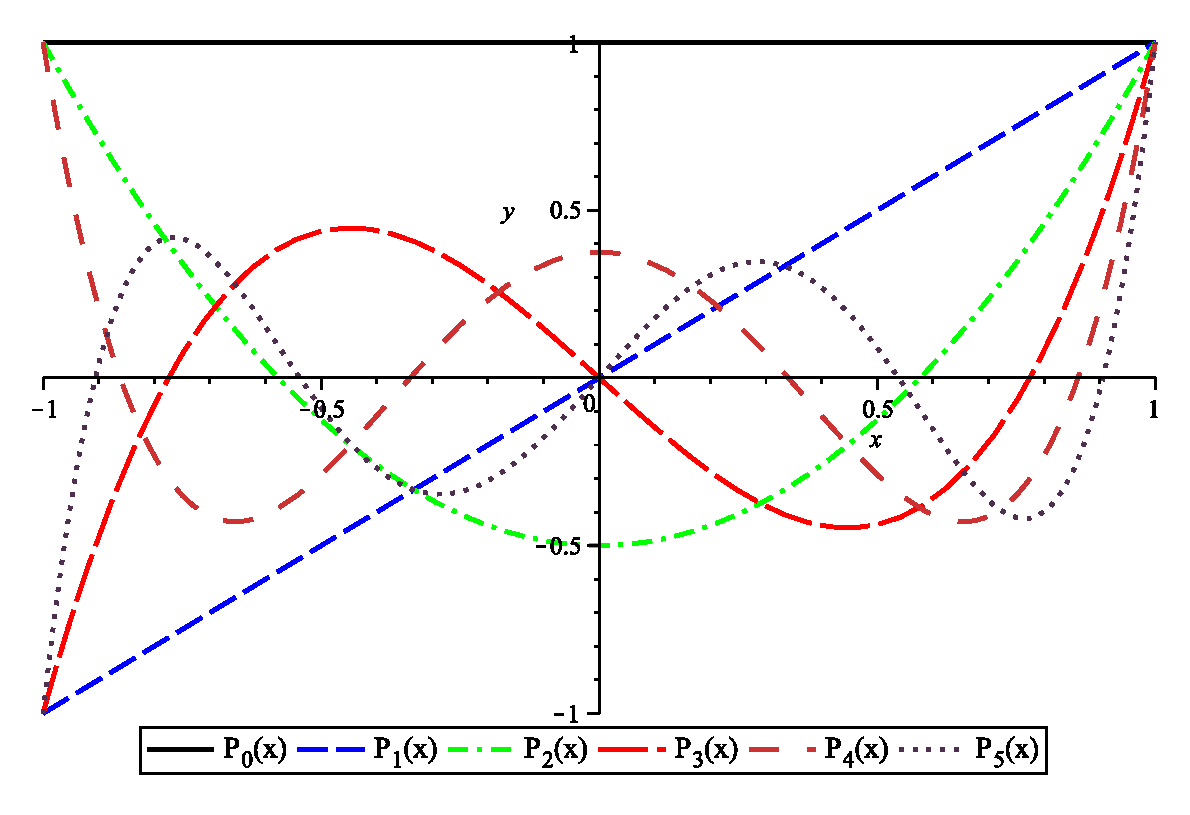
\includegraphics[keepaspectratio, width = 5.0 in]{images/legendre_polynomials}
    \caption{The first several Legendre polynomials, $P_N(x)$.}
    \label{fig:legendre_polynomials}
\end{figure}

The Legendre polynomials are useful for expanding the scattering cross-section because they are orthogonal over the range $-1 \leq \mu \leq 1$.  Moreover, expansions in the Legendre polynomials are unique in that the zeroth moment $\Sigma_{s0}$ preserves the integral properties of the underlying distribution (i.e the mean), whereas the other moments merely provide shape.  By looking at the $P_N$ in Figure \ref{fig:legendre_polynomials}, this becomes more obvious when one notes only $P_0$ has a non-vanishing integral over the domain.

\section*{Expanding the Angular Dependence}

To derive the $P_N$ equations, we must be careful to choose a starting point consistent with our expansion of the scattering kernel defined by Eqs. \ref{eq:scatterkernel} and \ref{eq:scattermoment}.  If we're not, it's easy to encounter a phantom $2\pi$!  Take as our starting point the monoenergetic transport equation in slab geometry with arbitary angular dependence of the scattering and source terms,
\begin{equation}
\begin{split}
 \mu \frac{\partial \psi}{\partial x} + \Sigma_t(x)\psi(x,\mu) &= \int^{2\pi}_0 d\phi' \int^1_{-1} d\mu' \Sigma_s(x,\mu_0)\psi(x,\mu')  + S(x,\mu)  .
\end{split}
 \label{eq:slabtransportequationgeneral}
\end{equation}

We expand the source
\begin{equation}
 S(x,\mu) = \sum^{\infty}_{n=0} \frac{2n+1}{4\pi} S_{n}(x)P_{n}(\mu) \, , 
 \label{eq:sourceexp}
\end{equation}
where
\begin{equation}
 S_{n}(x) = 2\pi \int^{1}_{-1} S(x,\mu) P_n(\mu) d\mu \, ,
\end{equation}
and the angular flux
\begin{equation}
 \psi(x,\mu) = \sum^{\infty}_{n=0} \frac{2n+1}{4\pi} \psi_{n}(x)P_{n}(\mu) \, , 
 \label{eq:psiexp}
\end{equation}
where
\begin{equation}
 \psi_{n}(x) = 2\pi \int^{1}_{-1} \psi(x,\mu) P_n(\mu) d\mu \, .
\end{equation}
% Substituting Eqs. \ref{eq:sourceexp} and \ref{eq:psiexp} along with Eq. \ref{eq:scatterkernel} into Eq. \ref{eq:slabtransportequationgeneral}, we find
% \begin{equation}
%  \begin{split}
%    & \mu \sum^{\infty}_{n=0} \frac{2n+1}{4\pi}P_{n}(\mu) \Big ( \frac{\partial \psi_n(x)}{\partial x} + \Sigma_t(x)\psi_n(x) \Big ) =  \sum^{\infty}_{n=0} \frac{2n+1}{4\pi} S_{n}(x)P_{n}(\mu) + \\
%    & \int^{2\pi}_0 d\phi' \int^1_{-1} d\mu'  \sum^{\infty}_{l=0} \frac{2l+1}{4\pi} \Sigma_{sl}P_{l}(\mu_0) \sum^{\infty}_{n=0} \frac{2n+1}{4\pi} \psi_{n}(x)P_{n}(\mu')    .
%  \end{split}
% \end{equation}
Before substituting these expressions, it helps to simplify the scattering expression.  Using Eq. \ref{eq:scatterkernel}, we can write the scattering term of Eq. \ref{eq:slabtransportequationgeneral}
\begin{equation}
\begin{split}
  \int^{2\pi}_0 d\phi' \int^1_{-1} d\mu'  & \Sigma_s(x,\mu_0)\psi(x,\mu')  \\
  &= \int^{2\pi}_0 d\phi' \int^1_{-1} d\mu'  \sum^{\infty}_{l=0} \frac{2l+1}{4\pi} \Sigma_{sl}(x)P_{l}(\mu_0) \psi(x,\mu') \, .
\end{split}
\end{equation}
Here, we make use of the \textit{Legendre addition theorem}, which states 
\begin{equation}
 P_l(\mu_0) = P_l(\mu)P_l(\mu') + 2\sum^l_{m=1}\frac{(l-m)!}{(l+m)!}P^m_l(\mu)P^m_l(\mu')\cos(m(\phi-\phi')) \, ,
\end{equation}
where $P^m_l(\mu)$ are the \textit{associated Legendre polynomials}, defined
\begin{equation}
 P^m_l(\mu) = \sqrt{(1-\mu^2)^m} \frac{d^m P_l}{d\mu^m} \, .
\end{equation}
Substituting this in, we find
\begin{equation}
\begin{split}
   \int^{2\pi}_0 d\phi' \int^1_{-1} d\mu'  & \sum^{\infty}_{l=0} \frac{2l+1}{4\pi}  \Sigma_{sl}(x)P_{l}(\mu_0) \psi(x,\mu') \\
  = \sum^{\infty}_{l=0} \frac{2l+1}{4\pi} & \Sigma_{sl}(x) \int^1_{-1} d\mu'  \psi(x,\mu')   \int^{2\pi}_0 d\phi' \Bigg ( P_l(\mu)P_l(\mu') + \\  
  & 2\sum^l_{m=1}\frac{(l-m)!}{(l+m)!}P^m_l(\mu)P^m_l(\mu')\cos(m(\phi-\phi'))\Bigg )\, .
\end{split}
\end{equation}
Noting that $ \int^{2\pi}_{0} \cos(m(\phi-\phi')) d\phi' = 0$, we find
 \begin{equation}
\begin{split}
   \int^{2\pi}_0 d\phi' \int^1_{-1} d\mu'  & \sum^{\infty}_{l=0} \frac{2l+1}{4\pi}  \Sigma_{sl}(x)P_{l}(\mu_0) \psi(x,\mu') \\
  = \sum^{\infty}_{l=0} \frac{2l+1}{4\pi} & \Sigma_{sl}(x) \int^1_{-1} d\mu'  \psi(x,\mu')   \int^{2\pi}_0 d\phi' \Big ( P_l(\mu)P_l(\mu') \Big ) \\
  = \sum^{\infty}_{l=0} \frac{2l+1}{4\pi} & \Sigma_{sl}(x)  P_l(\mu) \Bigg( 2\pi \int^1_{-1} d\mu'  \psi(x,\mu') P_l(\mu')\Bigg )  \\
  = \sum^{\infty}_{l=0} \frac{2l+1}{4\pi} & \Sigma_{sl}(x)  P_l(\mu) \psi_l(x)  \, .
\end{split}
\label{eq:simplescatter}
\end{equation}

Substituting the simplified scattering term of Eq. \ref{eq:simplescatter} and the expansions of Eqs. \ref{eq:sourceexp} and \ref{eq:psiexp} into Eq. \ref{eq:slabtransportequationgeneral} yields
\begin{equation}
 \begin{split}
   \sum^{\infty}_{n=0} &\frac{2n+1}{4\pi}P_{n}(\mu)  \Big (  \mu\frac{\partial \psi_n(x)}{\partial x} + \Sigma_t(x)\psi_n(x) \Big ) = \\
    & \sum^{\infty}_{n=0} \frac{2n+1}{4\pi}  \Sigma_{sn}(x)  P_n(\mu) \psi_n(x) + \sum^{\infty}_{n=0} \frac{2n+1}{4\pi} S_{n}(x)P_{n}(\mu) \, .
 \end{split}
 \label{eq:pnalmost}
\end{equation}
By rearranging the Legendre recurrence relation of Eq. \ref{eq:legpolyrecur}, we can express the product $\mu P_n(\mu)$ as
\begin{equation}
 \mu P_n(\mu) = \frac{1}{2n+1}\Big ( (n+1)P_{n+1}(\mu) + n P_{n-1}(\mu)\Big )\, .
\end{equation}
Substituting this in for $\mu P_n$ in the first term on the left of Eq. \ref{eq:pnalmost} and cancelling a few like terms yields
\begin{equation}
 \begin{split}
   \sum^{\infty}_{n=0} & \Bigg ( \Big ( (n+1)P_{n+1}(\mu) + nP_{n-1}(\mu) \Big )  \frac{\partial \psi_n(x)}{\partial x} + (2n+1)P_n(\mu) \Sigma_t(x)\psi_n(x) \Bigg ) = \\
    & \sum^{\infty}_{n=0} (2n+1) \Sigma_{sn}(x)  P_n(\mu) \psi_n(x) + \sum^{\infty}_{n=0} (2n+1)S_{n}(x)P_{n}(\mu) \, .
 \end{split}
 \label{eq:pnalmost2}
\end{equation}
To exploit the orthogonality property defined in Eq. \ref{eq:legpolyorth}, we multiply both sides of Eq. \ref{eq:pnalmost2} by $\frac{2m+1}{2}P_m$ and integrate the result over $-1 \leq \mu \leq 1$.  Then we find
\begin{equation}
 \begin{split}
   \int^{1}_{-1} d\mu \Bigg \{ \sum^{\infty}_{n=0} & \frac{2m+1}{2}P_m(\mu)\Bigg ( \overbrace{(n+1)P_{n+1}(\mu)\frac{\partial \psi_n}{\partial x}}^{\delta_{n+1,m}\to n=m-1} + \overbrace{nP_{n-1}(\mu)\frac{\partial \psi_n}{\partial x}}^{\delta_{n-1,m}\to n=m+1} \Bigg )   \Bigg \} = \\
   & m\frac{\partial \psi_{m-1}}{\partial x} + (m+1)\frac{\partial \psi_{m+1}}{\partial x} \, ,
 \end{split}
 \label{eq:pnalmost3a}
\end{equation}
and
\begin{equation}
 \int^{1}_{-1} d\mu \frac{2m+1}{2}P_m(\mu) (2n+1)P_n(\mu) \Sigma_t(x)\psi_n(x)  = (2m+1) \Sigma_t(x) \psi_m(x) \, ,
\end{equation}
and similarly for the scattering and source terms.  Together, we have
\begin{equation}
\begin{split}
 \frac{m+1}{2m+1}\frac{\partial \psi_{m+1}}{\partial x} &+ \frac{m}{2m+1}\frac{\partial \psi_{m-1}}{\partial x} +  \Sigma_t(x) \psi_m(x) = \\
  & \Sigma_{sm}(x) \psi_m(x) + S_m(x) \, , \, \, m = 0 \ldots \infty \, ,
\end{split}
\label{eq:pninfinite}
\end{equation}
where we take $\psi_{-1} = 0$.

\section*{The $P_N$ Equations}

Eq. \ref{eq:pninfinite} is an infinite set of coupled differential equations that represents an exact treatment in angle.  To yield a tractable problem, we make the $P_N$ approximation:
\begin{equation}
 \frac{d\psi_{N+1}}{dx} = 0 \, .
 \label{eq:pnapprox}
\end{equation}
As an example, the $P_1$ approximation yields
\begin{equation}
 \begin{split}
  n &= 0: \, \, \, \, \frac{d\psi_1}{dx} + \Sigma_t(x)\psi_0 (x) = \Sigma_{s0}\psi_0 + S_0 \\
  n &= 1: \, \, \, \, \frac{1}{3}\frac{d\psi_0}{dx} + \Sigma_t(x)\psi_1 (x) = \Sigma_{s1}\psi_1 + S_1 \, ,
 \end{split}
 \label{eq:p1approx}
\end{equation}
which is a set of two equations in the two unknown Legendre moments $\psi_0$ and $\psi_1$.  In general, the $P_N$ approximation gives $N+1$ equations in an equal number of unknowns.

An interesting fact is that the $P_N$ approximation is equalivalent to the $S_{N+1}$ approximation in slab geometry if the Gauss-Legendre quadrature set is used, proof of which is left as an exercise for the simple case of the $P_1$ and $S_2$ equations.  A similar equivalence can me made in certain cases for higher dimensions between the spherical harmonics equations and multidimensional $S_N$ approximations.  Doing so is one way to mitigate the numerical artifacts known as ray effects common to the $S_N$ approximation.  See the references in the Further Reading.

\section*{Diffusion Theory}

The $P_N$ equations give us one formal way to derive the diffusion equation.  Suppose in Eq. \ref{eq:p1approx} that we take the source to be isotropic so that $S_1 = 0$.  Moreover, we define the first scattering momement to be $\Sigma_{s1} = \Sigma_{s0}\bar{\mu}$, where $\bar{\mu} = \int^1_{-1}d\mu \mu \Sigma_s(\mu) / \int^1_{-1} d\mu \Sigma_s(\mu)$.

Then, we rearrange Eq. \ref{eq:p1approx} to find
\begin{equation}
 \psi_1 (x) = \frac{-1}{3(\Sigma_t - \Sigma_{s0}\mu)} \frac{d\psi_0}{dx} \equiv -D(x) \frac{\psi_0}{dx} \, ,
\end{equation}
so that 
\begin{equation}
 -\frac{d}{dx} D(x) \frac{\psi_0}{dx} + (\Sigma_t - \Sigma_{s0})\psi_0(x) = S_0 (x) \, .
\label{eq:neutrondiffusion}
\end{equation}
This is the diffusion equation, and we recognize $\psi_0(x)$ as the scalar flux $\phi(x)$, $\psi_1(x)$ as the current density $J(x)$, and $D$ as the diffusion coefficient.  Note that while diffusion theory explicitly assumes an isotropic source, it does treat linearly anisotropic scattering exactly.

\section*{Boundary Condition}

In general, there are two approaches to defining boundary conditions for the $P_N$ (or diffusion) equations:
\begin{enumerate}
 \item conserve net current (Marshak)
 \item obtain correct boundary flux for a finite number of $\mu$ values (Mark)
\end{enumerate}
The $P_N$ approximation consists of $N+1$ equations, which requires $N+1$ boundary conditions.  Typically, it's desirable to spread these conditions evenly among surfaces.  For a slab system, there are just two surfaces, and for odd $N$, there are an even number of conditions to be satisfied.  Hence, we typically only use odd $N$ approximations.

\section*{Marshak Conditions}

The \textit{Marshak} condition places a limit on the odd moments of the $P_N$ expansion, as the odd moments drive net flows in angular space.   Suppose we are given an incident boundary condition $B_L(\mu)$ on the left hand side, represented as
\begin{equation}
 \psi(x_L,\mu) = B_L(\mu) \, , \,\,\, \mu > 0 \, .
\end{equation}
Then the Marshak condition states
\begin{equation}
 \int^1_0 \psi(x_L,\mu)P_l(\mu)d\mu = \int^1_0 B_L(\mu) P_l(\mu)d\mu  \, ,
\end{equation}
for $l = 1,\, 3,\, \ldots \, ,N$.  In general, the Marshak conditions give the best results for the $P_N$ equations.  Moreover, they capture the physically appealing notion of conservation of particles across the boundary.

\section*{Mark Condition}

The Mark condition can be expressed as
\begin{equation}
 \psi_l(x_L) = \int^1_{-1} B_L(\mu) \delta(\mu-\mu_n)P_l(\mu) d\mu = B(\mu_n) P_l(\mu_n) \, ,
\end{equation}
for a desired set of $\mu_n$.  Typically, these $\mu_n$ are chosen to be symmetric for an equal number of $\mu_n$ per half-space.   A common choice are the $\mu_n$ such that $P_{N+1}(\mu_n) = 0$, which should look strikingly similar to the condition for generating abscissa for the Gauss-Legendre quadrature set.

\section*{A Simple Code}
To be continued.

\section*{Further Reading}
To be continued.

\begin{exercises}

  \item  \textbf{P$_{\mathbf{1}}$ Boundary Conditions}. Derive the $P_1$ equations for isotropic scattering and an isotropic source.  Derive the Marshak vacuum conditions for arbitrary left and right boundaries in a slab.  Do the same for the Mark conditions. 

  \item \textbf{P$_{\mathbf{2}}$ Equations}. Show for the case of linearly anisotropic scattering and isotropic source that the $P_2$ equations can be written as a second order partial differential equation similar in form to the typical neutron diffusion equation.

  \item \textbf{Numerical Solution of the P$_{\mathbf{1}}$ Equations}. Consider a slab of width 10 cm with $\Sigma_t = 1.0$ [cm$^{-1}$], and $c = \Sigma_s / \Sigma_t = 0.5$ (isotropic scattering in the lab system).  A uniform, isotropic source of $1$ [n/cm$^2$-s] is located in the first half of the slab, and both slab edges are subject to vacuum conditions. Write a code to solve the $P_1$ approximation to this problem using Marshak conditions.  Plot $\psi(x,\mu)$ at $x = 0$, $2.5$, $5.0$, $7.5$, and $10$ [cm].  Plot $\phi(x)$ over the whole slab.

  \item \textbf{Numerical Solution of the P$_{\mathbf{3}}$ Equations}. For the same problem, write a code to solve the $P_3$ approximation using Marshak conditions.

  \item \textbf{ Diffusion via asymptotics}.  Consider the following rescaling of the 1-d, mono-energetic transport equation with isotropic scattering. Finish me.

  \item \textbf{Legendre Addition Theorem}. Prove the Legendre polynomial addition theorem.  You may use any resource you want, but make sure you understand all steps of the proof.  A particularly straightforward approach begins as follows.  Start with an expansion of an arbitrary function in the full spherical harmonics.  Then, substitute the definition of the expansion coefficients back into the expansion.  Noting that the integral and summation can be switched, what function must the summation be?  

  \item \textbf{Defining the Scattering Angle}. Prove $\mu_0 = \cos(\theta)\cos(\theta')+\sin(\theta)\sin(\theta')\cos(\phi-\phi')$, where $\mu_0$ is the cosine of the scattering angle and ($\theta$,$\phi$) and $(\theta',\phi')$ are the original and final angles, respectively.  Include a diagram.

\end{exercises}
